\graphicspath{{./Ch1-Introduction/images/}}

\chapter{Introduction} \label{chap:introduction}
\begin{comment}
//clearly come out what are you doing in this thesis and what are the contributions
//what field you are targetting, scope and motivation, what problems, to justify your contributions.
1. About AI/ML/NN/DNNs: Applications, Domains, Growth, Type of NNs, Training and inference, 

2. Modern DNNs, architectures and popular NNs

3. Example: Number of computations, parameters: Illustrate compute and memory intensive operations.
Number of layer

4. Edge vs. Cloud Computing. 

5. Edge AI Challenges

6. About the Architectures for Edge AI Accelerators: Give wider scope of these architectures, and specific type of architectures. Trade-offs.

7. Performance bottlenecks for edge AI: Memory and Throughput bottlenecks.
Memory accesses are the key botllenecks for these edge AI devices. 

6. Summary and Outline of the Thesis.

\end{comment}

The past few years have seen exponential growth in Neural Network (NN) based applications. NN applications are widely used in healthcare, agriculture, road safety, surveillance, defense, number plate identification, medical diagnosis, autonomous driving, recommender systems, and many more. Modern computing systems capable of storing and processing large volumes of data and the availability of big data sets due to digitization have enabled NNs to achieve human-like performance, which was not possible a few decades ago. Their growth was also accelerated by the software libraries like Tensorflow and PyTorch that provide ease of development.

Today, NN-based applications have penetrated our daily lives, e.g., face recognition for authentication, chatbots, shopping recommendations, and photo tagging. Their unprecedented success in solving complicated real-world problems has increased their usage in embedded systems ranging from smartphones and tablets to wearable devices. NNs are also used in the clinical environment, e.g., in bacterial identification and tumor detection. Several of these devices need to be mobile, battery-operated, and should have lightweight. Often, such systems have limited computing resources and tight energy-budget. With time, NNs are growing in size to solve complicated problems and improve accuracy; this trend is expected to continue for several years.  

\section{Neural Network Model}
Neural Networks are machine learning algorithms inspired by processing mechanisms in the human brain. They can learn from the data using a training process without being programmed explicitly. Inspired by the brain, NNs consist of several neurons connected and organized as layers. There can be several hidden layers in a NN. \figref{fig:simpleNN} shows a simple NN example. 
\begin{figure}[!htb]
	\centering
	\captionsetup{font=sf}
	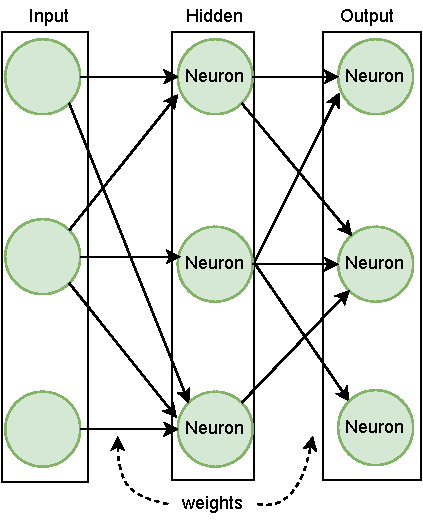
\includegraphics[width=0.3\textwidth]{simpleFFNN}
	\caption{Example of simple Neural Network.}
	\label{fig:simpleNN}
\end{figure}

Several classes of NNs exist that differ in the number of neurons, connections between them, and training method. Broadly they can be classified as feedforward neural networks (FFNNs) and recurrent neural networks (RNNs) based on the flow on the flow of data between layers. Convolutional Neural Networks (CNNs) and Long short-term memory networks (LSTMs) are quintessential examples of FFNNs and RNNs, respectively. CNNs are mainly used in computer vision-related applications like image classification and object detection, and LSTMs are used in sequential data processing applications like speech recognition and natural language processing (NLP). 

On one hand there are single-layer NNs that consist of just two layers - an input and an
output layer, with only the output layer performing the computation. Self-Organizing
Maps (SOMs) are examples of single-layer NNs and are used in dimensionality reduction
and clustering applications. On the other hand, there are modern NN architectures that
are very deep and involve many layers and millions of parameters. Multilayer NNs with
more than three layers are referred to as deep neural networks (DNNs). These DNNs
are capable of learning complex functions from the data.

\section{Phases of NN Applications: Development to Deployment}
NNs need not be programmed explicitly, and they learn from the raw data to provide solutions to real-world problems. For example, NNs first learn to classify an object in an image, in which several example images are provided. This learning process is referred to as training. Once trained, the NN can estimate the output for a new input. Subsequently, the trained NNs are used in applications to estimate the new input's output. This phase is referred to as inference.

\figref{fig:workFlow} shows difference phases of NNs from development to deployment. The development phase is usually performed on desktop/laptop machines using deep neural network frameworks, e.g., PyTorch and TensorFlow. 
\begin{figure}[!htb]
	\centering
	\captionsetup{font=sf}
	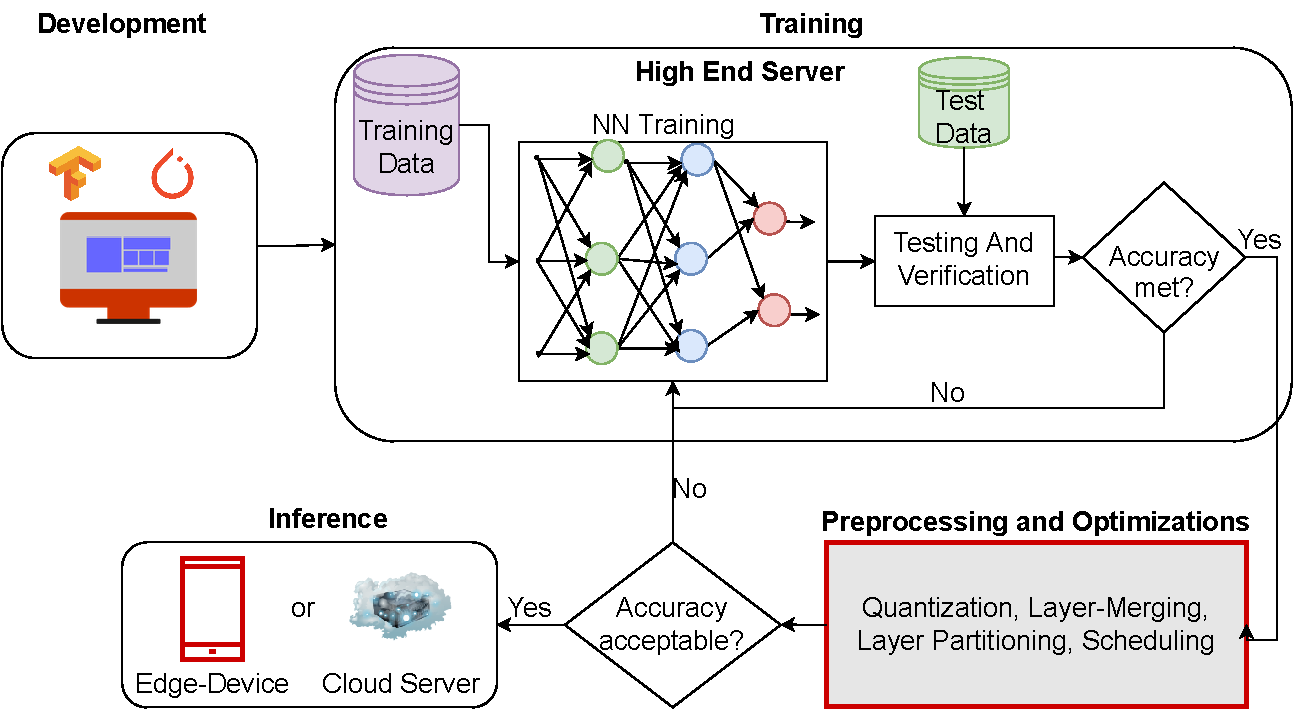
\includegraphics[width=0.8\textwidth]{WorkFlow}
	\caption{Work Flow for Neural Networks.}
	\label{fig:workFlow}
\end{figure}
After the development phase, NNs undergo a training phase where they learn from examples. These DNNs require large training data sets for learning and must go through multiple iterations to achieve the desired accuracy. Training of NNs involves updating weights and biases using large input samples. It is a repetitive process until the desired accuracy is achieved. Training a DNN may last from a few hours to several weeks. Hence training of DNNs is generally performed on high-performance systems, typically using GPUs. 

After the training phase, trained models are used in applications for inferencing, where the deployment platforms may range from cloud to embedded devices. Inference phase computations also involve millions of computations and access large volumes of data. For example, a popular CNN, VGG16, performs 15.47 GMAC operations and accesses 138 million parameters for a single inference. If the NNs are deployed on the cloud, the throughput and energy demands can be met using high-performance systems like GPU. However,  deployment on edge devices is challenging due to limited energy and computing resources. Hence optimizing these models before inferencing on edge devices is a must. In this work, we focused on optimizing NN models before deployment on edge devices for inferencing. This phase is shown as \textbf{Preprocessing and Optimization} block in \figref{fig:workFlow}.

\section{Edge AI: Inferencing on Edge Devices}
Edge devices are battery-operated with limited resources and a tight energy budget. A few years back, edge devices were primarily used to collect real-world data, and inferences were performed on the cloud. There is a growing trend of shifting the processing of these DNN applications from the cloud to edge devices near the sensors as it improves the user experience, eliminates network bandwidth issues, and improves privacy and security. 

Today we see an explosion of applications using deep learning algorithms in consumer electronic devices. Manufacturers are shifting the processing of NNs from cloud to edge devices.  Several latest consumer electronic devices, like smartphones, digital cameras, etc., are already equipped with NN applications. 

However, DNN inferencing on edge devices is challenging. \figref{fig:edgeAIChallenges} shows the key challenges for Edge AI devices. Energy efficiency and throughput are the two most important metrics for edge devices. While energy efficiency is paramount for longer battery time, high throughput is desired for better user-response time. Efficient processing of DNNs inferencing on edge devices is critical for their widespread usage. 

\begin{figure}[!htb]
	\centering
	\captionsetup{font=sf}
	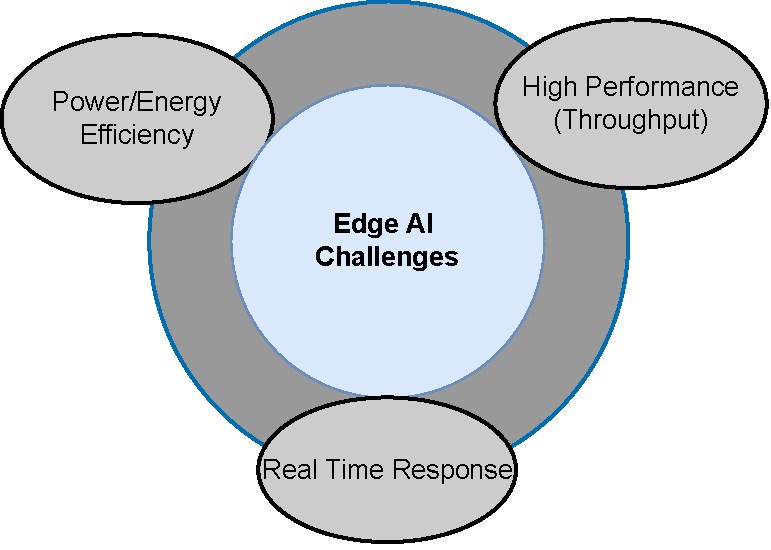
\includegraphics[width=0.6\textwidth]{edgeAIChallenges}
	\caption{Key challenges for Edge-AI Accelerator}
	\label{fig:edgeAIChallenges}
\end{figure}
%\subsection{NN Accelerators}
Edge devices use customized NN accelerators to meet energy and throughput demands. \figref{fig:typicalDNNAccelerator} shows a typical DNN accelerator architecture, which consists of an off-chip memory and an accelerator chip. An accelerator chip mainly consists of an on-chip memory of a few hundred KBs and an array of Processing Elements (PEs). The accelerator system has multiple memory levels: off-chip memory, on-chip memory, and the registers inside the PEs. Each memory level has a different storage capacity, access latency, and energy costs. The access energy from off-chip memory is up to two orders of magnitude higher than a PE computation operation~\cite{Chen2016EyerissAS}. 
\begin{figure}[!htb]
	\centering
	\captionsetup{font=sf}
	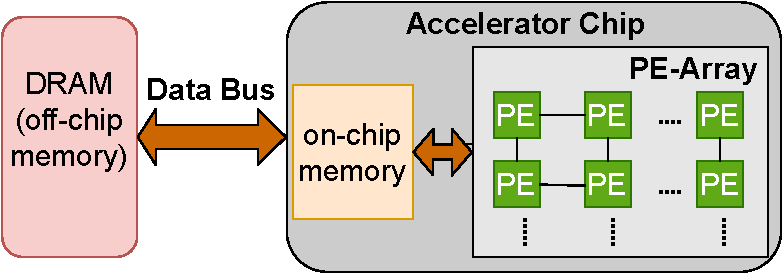
\includegraphics[width=0.7\textwidth]{typicalDNNAccelerator}
    \caption{Typical DNN accelerator architecture.}
   	\label{fig:typicalDNNAccelerator}
    \vspace{1.0em}
\end{figure}

In this thesis, we aimed to improve edge NN accelerators' performance and energy efficiency during the inference phase.

\section{Energy Efficient NN Inferencing}
\subsection{Previous Work}
Several FPGA~\cite{zhang2015optimizing,wei2019overcoming,gokhale2014240,8742284,gupta2015deep,alwani2016fused}, GPU~\cite{chetlur2014cudnn} and ASIC~\cite{Chen2016EyerissAS,chen2014diannao,chen2014dadiannao,du2015shidiannao} accelerators have been proposed to meet the performance and energy targets. These accelerators apply different techniques to speed up operations. NN computations are memory intensive. With limited on-chip memory on the accelerators and a large difference between latencies and energy consumption of off-chip and on-chip memories, off-chip memory accesses dominate the performance and energy consumption of these accelerators. As much as 80\% of the overall energy consumption
of an NN accelerator could be due to off-chip memory accesses~\cite{chen2014diannao}. Therefore, reducing the off-chip memory is the key to improving the throughput and energy efficiency of DNN accelerators. This has led several researchers to focus on reducing the off-chip
memory accesses~\cite{chen2014diannao,chen2016eyeriss,zhang2015optimizing}. Some approaches~\cite{lee2016fpga, rybalkin2018finn, ferreira2016fpga} have used on-chip memory to
store all the weights. However, since sizes of weights in modern NN models can be several MBs, these approaches are not scalable and are effective only for small NN models. Approaches attempting to reduce the off-chip memory accesses of NN accelerators can be classified into two broad categories, as shown in \figref{fig:previousWorkClassification}. 

\begin{figure}[!htb]
	\centering
	\captionsetup{font=sf}
	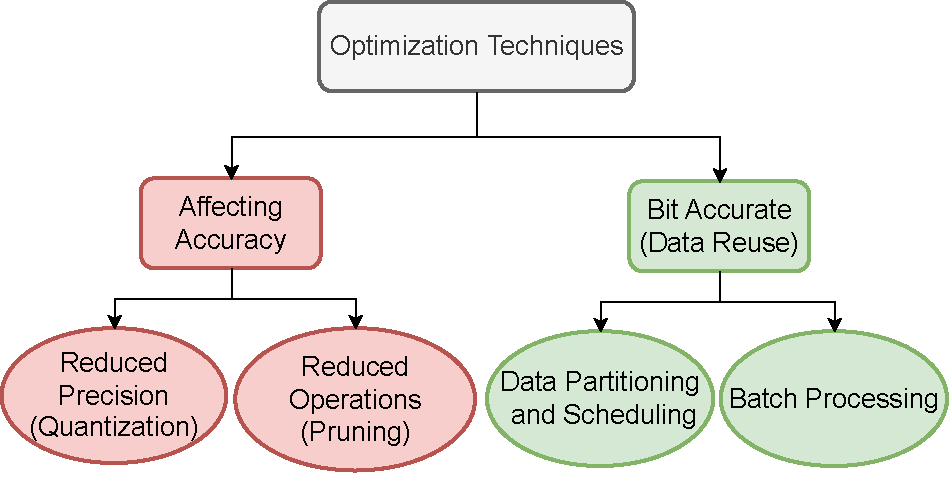
\includegraphics[width=0.7\textwidth]{previousWorkClassification}
	\caption{Broad Classification of previous works for improving the performance of DNN accelerators.}
	\label{fig:previousWorkClassification}
\end{figure}

One category of work exploits error-tolerance and redundancy in NNs using quantization, compression, and pruning techniques to reduce the precision, the number of operations, and models' size~\cite{ferreira2016fpga,wang2018c,chang2015recurrent,han2017ese,lee2016fpga}. With reduced precision, the storage requirement and memory accesses reduce proportionally and improve energy efficiency~\cite{sze2017efficient}. Quantization and pruning techniques result in reduced NN model sizes. The reduced model for shallow NNs may fit into the on-chip memory and thus eliminate the off-chip memory bandwidth bottleneck. However, quantization and pruning approaches impact the accuracy of the networks and may only be suitable where accuracy can be compromised. These techniques have been explored only for limited domains such as image
processing and computer vision. The number of parameters in modern DNNs is significantly large. For these DNNs, besides quantization and pruning, additional techniques may be required to reduce the off-chip memory accesses further.

The second category of approaches that do not affect the accuracy of the network are data-
reuse schemes. The data-reuse schemes are orthogonal to the quantization techniques and can be combined to reduce off-chip memory accesses further. These schemes aim to reduce repeated off-chip accesses to the same NN coefficients when the entire set of NN coefficients does not fit in the on-chip memory. This is quite effective for many modern DNNs (e.g., CNNs, RNNs) with a significantly large number of parameters. One popular scheme which reuses weights is batch processing~\cite{zhang2015optimizing,Li2018SmartShuttleOO,que2019efficient}. During the inference phase, all the inputs use the same weights. In the batch processing scheme, inputs are grouped as a batch and processed to reuse the weights from the on-chip memory. Increasing the batch size improves the weights reuse but increases the latency, which is undesirable. Secondly, the batch processing scheme only improves the weights reuse, and other layer data types do not get the benefit.

Another well-known data reuse technique is data partitioning and scheduling~\cite{zhang2015optimizing, Li2018SmartShuttleOO}. In this technique, the data is partitioned into tiles, and operations are scheduled so that data can be accessed from the on-chip memory as far as possible. Modern CNNs have layer data sizes too large to fit into on-chip memory, and it is essential to partition the layer data. There are numerous ways of data partitioning and scheduling for a given CNN layer, offering different extents of data reuse. Choosing an optimal way here is non-trivial.

Loop tiling is applied to partition the layer data, a well-known compiler technique~\cite{aho2006compilers}. Conventional problems apply loop tiling where equal data-reuse opportunities exist in all the data dimensions. However, in CNN layers, there are multiple types of data reuse, and the extent of each data reuse varies with different dimensions. Increasing tile dimensions to improve one type of data reuse reduces other types. It is important to consider all the possible types of data reuses of a layer to find the optimal solution. Deciding on the optimal partitioning of NN layers is more challenging than conventional problems.

Compared to FFNNs, RNN computations pose a different challenge for data reuse. RNNs have feedback connections that result in dependency on previous time step computations and limit the possible data reuse. Due to limited on-chip memory of accelerators, the weights are repeatedly accessed from the off-chip memory at each time step. This results in a large volume of off-chip memory access. Que et al.~\cite{que2019efficient} proposed a blocking-batching scheme. However, the benefit of their scheme is limited to matrices involved in time-step independent computations. To handle the dependency problem, Park et al.~\cite{park2020time} proposed a time-step interleaved weight reuse scheme (TSI-WR) that reuses the weights in a time-interleaved manner. However, their approach was only partially able to reuse the data, and the extent of reuse depends on the on-chip buffer sizes. Their approach is effective for accelerators with sizeable on-chip memory.
\subsection{Thesis objectives and contributions}
The objective of this thesis has been to provide novel energy-efficient solutions for NN accelerators by reducing off-chip memory accesses. The proposed techniques fall within the classification of \figref{fig:previousWorkClassification} but carry some new ideas. Since every memory access reduction technique is not necessarily applicable to the entire range of NN algorithms, we have considered three NN algorithms that present quite different characteristics from each other. These are Self Organizing Maps (SOMs), Convolutional Neural Networks (CNNs) and Recurrent Neural Networks (RNNs).

We have applied quantization techniques on Self Organizing Maps (SOMs) to analyze the
impact on NN accuracy and the benefits of improving energy efficiency. These are single layer
FFNNs have not been studied in this context previously. We hand-crafted a custom semi-systolic array design for different bit width implementations to analyze the accuracy versus energy trade-off for SOMs. 

For multilayer feedforward and recurrent NNs, we have proposed novel data reuse approaches. To find energy-efficient solutions, estimating the off-chip memory accesses is essential. Performing the measurements on the hardware is time-consuming, and vast design space makes it practically impossible. From the description of the NN layer, it is not easy to estimate the off-chip memory accesses. Several factors impact the off-chip memory accesses of the NN layer, which were not considered by the previous works, e.g., bus width and address alignment. In this work, we have developed an analytical framework that computes the off-chip memory accesses of 3D data partitioned into small tiles. The analytical framework considers data shape, tile dimensions, accelerator architecture parameters, and data resolution to compute the off-chip memory accesses.

For CNNs where partitioning and scheduling scheme makes a significant impact, we have analyzed memory accesses of various partitioning and scheduling schemes for memory-intensive layers. There are several possible ways to partition the layer data and schedule the operations of DNN layers. We expressed determining the optimal solution that minimizes off-chip memory accesses of a NN layer as a constraint optimization problem. We have developed and integrated a model with the analytical framework for computing the off-chip memory accesses of different CNN layers. Previous approaches~\cite{zhang2015optimizing, Li2018SmartShuttleOO} have ignored the architectural parameters while determining the optimal solution. Our objective in this work is to analyze the impact of architectural parameters on overall off-chip memory access of CNN accelerators and use that information to determine the optimal tile dimensions to reduce the accesses and the total energy of the CNN accelerators.

We implemented the hardware design for memory-intensive CNN layers on FPGA to measure the off-chip memory accesses, latency, run-time, and design power. The implementation is configurable for layer shapes, tile dimensions, on-chip memory sizes, bus width, and data resolution. We measured the energy efficiency and throughput of different approaches using the FPGA design and validated the results of the analytical framework.

Besides CNNs, the other popular class of NN is RNNs. The main challenge in optimizing the off-chip memory accesses of RNNs is the dependency on previous time-step computations. If the accelerator's memory is not large enough to hold weight matrices, this results in a large volume of data accesses from the off-chip memory. To address this, we proposed a novel data reuse approach that reuses all the weights of such matrices for the two consecutive time steps. A characteristic of the proposed approach is that the extent of data reuse is independent of the accelerator's on-chip memory size, making it suitable for LSTM accelerators with small on-chip memory. We implemented the hardware design for LSTMs on FPGA for the proposed, conventional, and state-of-the-art data-reuse approaches. Using the FPGA designs, we estimated the energy efficiency and throughput and demonstrated the efficacy of our approach for popular LSTM models.
\section{Summary and Outline of the Thesis} 
Previous research has shown that for data partitioning and scheduling, making a choice independently for each layer of a NN is better than making a common choice for the entire NN because of the different shapes of various layers. We observe that the choice of optimal data partitioning and scheduling depends on the shape of a layer and architectural parameters. We present an analytical framework in \chapref{chap:analyticalFw} that quantifies the off-chip memory accesses for DNN layers of varying shapes, considering the architectural constraints. It helps compare different data partitioning and scheduling schemes to explore the large design space to find the optimal solution for improving the energy and throughput. 

Based on the above analytical framework, in \chapref{chap:CNN}, we propose a data reuse approach that considers the architectural parameters and determines the optimal partitioning and scheduling scheme to minimize the off-chip memory access of CNN layers. We demonstrate the efficacy of our partitioning and adaptive scheduling approach on the compute and memory-intensive CNN layers. 

\chapref{chap:RNN} proposes a novel data reuse approach to improve the throughput and energy efficiency of state-of-the-art recurrent neural networks (RNNs). The proposed approach splits the computations and combines them in a way that significantly reduces the off-chip memory accesses of large matrices. We measure the design power and memory accesses on FPGA implementation of Long-Short Term Memory Network (LSTM) accelerators and show our approach's energy and throughput improvements.

We analyze the effect of using different bit resolutions on the accuracy of a NN and the benefits of it for self-organizing maps (SOMs) for designing energy-constrained systems where the area, power, and performance are of critical importance in \chapref{chap:SOM}. Using an efficient implementation of SOM design on FPGA, which can be configured for different bit resolutions, we show performance comparison for different data precisions. 

The work done in this thesis improves the state-of-the-art of energy efficient execution of modern NNs and also gives directions to future research. In \chapref{chap:Conclusion}, we discuss these new research directions together with the conclusion of our work.